\documentclass[final]{svjour2}
\usepackage{amsmath}
\usepackage{graphicx}
\usepackage{rotating}
\usepackage{amssymb}
\usepackage{mathptmx}
\usepackage[numbers]{natbib}
\usepackage{float}
\usepackage[section]{placeins}
\usepackage{tabularx}
\usepackage{booktabs}
%\usepackage[nofighead,nomarkers]{endfloat}
\makeatletter
\journalname{Journal of Low Temperature Physics}
%%%%%%%%%%%%%%%%%%%%%%%%%%%%%% Textclass specific LaTeX commands.
%%%%%%%%%%%%%%%%%%%%%%%%%%%%%% User specified LaTeX commands.
\bibpunct{}{}{,}{s}{}{,}

\begin{document}

\newcommand{\hdblarrow}{H\makebox[0.9ex][l]{$\downdownarrows$}-}
\title{Design Considerations for Cryogenic Support Structures}

\author{E. Kramer \and N. Kellaris  \and M. Daal \and N. Zobrist \and S. Govindjee \and B. Sadoulet \and S. Golwala \and M. Hollister}

\institute{Department of Physics, U.C. Berkeley,\\ Berkeley, CA 94709, USA\\
\email{ekramer@berkeley.edu}}

\date{07.15.2013}

\maketitle

\begin{abstract}

Design specifications for the support structures of low temperature instrumentation often call for low thermal conductivity between temperature stages, high stiffness, and specific load bearing capabilities.  The challenge is usually to find a design that minimizes heat transfer along the structure while meeting strength and rigidity specifications.  Common design solutions employ thin-walled tubes and truss structures. In this contribution, we suggest, analyze and test several design approaches that incorporate such structures. In addition, we present some equations for failure modes and structural stiffness testing results.

\keywords{Truss, Thin-walled tube, Cryogenic Tower}

\end{abstract}

\section{Introduction}
Both slender member truss and thin-walled tube structures exhibit desirable qualities for low temperature instrumentation support structures due to their high structural stiffness to low thermal exchange across temperature stages.  Designing optimal structures that obtain the lowest thermal connection between stages while still remaining structurally adequate to support both forces while in use and while handling is a processes of optimization.  Theoretical equations and computer simulation of structural stiffness allow one narrow down possible design choices without needing to fabricate and physically test each design iteration.  While highly useful, calculations and computer simulations are not sufficient on their own. In the lab under non-ideal circumstances, materials and structures typically fail before their theoretical yield or break point due to imperfections, including but not limited to impurities in the material (microscopic fractures or holes), and misaligned or misshapen elements of the overall design.  Due to this, physical strength testing of a fabricated piece can be performed to confirm failure modes as well as discover unexpected ones.  Results from such tests allow one to better obtain the performance and factor of safety desired for the part being designed.

\section{Theory and Experimental details}
For this experiment, we began with theoretical analysis via computer simulation and then proceeded to fabricate and physically test a few promising designs.  Our truss structure analysis was performed using a matrix application of the method of joints.  In this technique all forces in truss members were assumed to be normal to their direction.  The forces at each node connecting truss members were statically determined using a system of equations, the boundary conditions (fixed, clamped, free), connectivity, and external loading.  This method allows us to solve for the forces along every the truss member (tension or compression) as well as all of the reaction forces on the fixed pin joints for a given stable and statically determinable structure.  Using these solutions and the material properties of the truss members, failure points were identified for each truss member, giving the structure an overall point of failure at when its weakest member fails.  The external force used for analysis was a shear/bending force where one end was assumed to be fixed while the other was subjected to a load perpendicular to the normal axis of the tower structure in order to create a cantilever beam scenario.  
Tube analysis was done using the model presented by Govindjee ([1]) which predicts failure in tube structures based off of their material composition as well as radial and thickness dimensions. The load was also assumed to be that of a simple bending cantilever beam setup as this is the most expected force to lead to failure in the Soudan tower.  Given a radius $a$ and a thickness $t$, the model considers four failure modes, shear instability, bending instability, material failure from normal stresses, and material failure from shear stresses.  Shear instability occurs when the maximum shear stress exceeds the critical torsional stress due to a purely torsional load.  This critical load ($P_{c}$), the point at which any loads above it will cause failure can be found using:

\begin{eqnarray}
P_{c}^{s} = \frac{\pi^3E}{12(1-\nu^2)^{-\frac{5}{8}}}a_{s}\frac{a^{1/4}t^{9/4}}{L^{1/2}}
\end{eqnarray}

Buckling instability takes place when the maximum compressive stress anywhere in the thin walled tuve exceeds a critical value.  By approximating the wall of a tube as a membrane the maximum stress in the tube is given by $\sigma_{b} = PL/a^2t\pi$. This leads us to a critical stress value given by Ba$\check{z}$ant [3].

\begin{eqnarray}
\sigma_{c}=\frac{E}{\sqrt{3(1-\nu^2)}}\frac{t}{a}.
\end{eqnarray}

We can then take this critical stress value and transform it into a critical load for localized buckling:

\begin{eqnarray}
P_{c}^{b} = \frac{E \pi}{\sqrt{3(1-\nu^2)}}\frac{t^2a}{L}
\end{eqnarray}

More straightforward than buckling, a tube can also fail just from exceeding its maximum normal stress. This occurs when the force applied is greater than the critical normal stress value ($P_{c}^{mn}$) determined by $\sigma_{f}$, the normal stress limit:

\begin{eqnarray}
P_{c}^{mn} = \sigma_{f} \pi \frac{a^2t}{L}
\end{eqnarray}

The last failure mode examined for tubes was that when the tube exceeds its shear stress limit $\tau_{f}$. Brittle material can typically be approximated by $\tau_{f} = \sigma_{t}\sqrt{R/3} $ where $R = \sigma_{c}/\sigma_{t}$ (compressive/tensile) while ductile materials have $\tau_{f} \approx \sigma_{f}/2 \ \text{or} \ \sigma_{f}/\sqrt{3}$ [4].

\begin{figure}[!ht]
\begin{center}
\includegraphics[%
  width=0.9\linewidth,
  keepaspectratio]{SW}
\end{center}
\caption{Our hexapod truss structure design (left) and a simple thin walled tube design (right)}
\label{SW}
\end{figure}

Using these theoretical results as guidelines, we then fabricated a few promising designs (shown above), including a hexapod truss structure and several pure thin walled tubes. These fabricated parts were then subjected to loads and the results were compared to the theoretical ones found previously.  Strength testing was done on a single axis machine with tension and compression capabilities. Samples were fitted to be able to be locked into the machine both along their center axis as well slightly off axis in order to test both tensile and compressive strength in the on axis and off axis.  An external frame was also used to allow our samples to be mounted horizontally, either supported as a pair of cantilever beams or a single simply supported beam, to be tested for pure shear and bending stiffness respectively.  We tested four sample types consisting of three truss structures and one thin-walled tube structure.  All three truss structures were identical in overall design, utilizing six members to connect two copper or aluminum hexagons base plates.  We tested three different types of truss members which included two Graphlite of 40 and 80 mil cross sectional diameters and one Titanium rectangular cross section member. The thin-walled tube structures were constructed from a single two inch length of two inch outside diameter Vespel tube connected with Stycast 1266 to two gold-plated copper baseplates. Two SP1 and SP22 10 mil wall thickness truss tube members were also fabricated to test on their own.

\section{Results}
Currently simulation and testing has been completed on the 40 and 80 mil hexapod truss structures under a pure bending load and on the SP1 and SP22 tubes in tension.  

(INSERT MACHINE SETUP PICTURE HERE)

All samples were tested to failure in a strain controlled environment.  The pull rate was 0.5 mm/sec for all tests.  Results of the four tests in a plot of stress vs strain is presented below.

\begin{figure}[!ht]
\begin{center}
\includegraphics[%
  width=0.65\linewidth,
  keepaspectratio]{Test}
\end{center}
\caption{The stress and strain vs time of four strength tests. 40 mil Graphlite hexapod in pure bending (top-left), 80 mil Graphlite hexapod in pure bending (top-right), 10 mil wall thickness SP1 tube truss member in tension (bottom-left), and 10 mil wall thickness SP22 tube truss member in tension (bottom-right).}
\label{Test}
\end{figure}

Results of these tests fit our expectations.  The SP1 and SP22 tube structures, being brittle materials, failed in due to exceeding their respective maximum normal stresses.  Their failure point came well before their simplified theoretical value however due to the small ventilation holes in their side for use in a vacuum environment.  Upon examination of the fracture surface, the failure propagated from this hole as its starting point, which is to be expected as circular holes in materials create localized stress concentrations of approximately 3.04 times greater than the stress elsewhere in the structure.  The hexapod structures, while not pushed to fracture failure, also reacted in the predicted way.  While our program successfully predicted which members would be put in tension and compression as well as which member would buckle and fail first, the model results were slightly off on the displacement of the overall structure.  The 40 mil structure was predicted to displace 3.175 mm under the maximum load we applied of 250 N (125 on each tower structure) but only displaced 0.5 mm when that force was reached. Each 80 mil structure was calculated to displace 12.7 mm at the maximum applied force of 1150 N across two tower structures.  Our data reveales that at that maximum point, each tower had only displaced apprloximatly 4 mm.  These discrepancies are most likely due to the approximations in our program about truss structure joints.  We assumed an ideal truss structure with all joints that are not fixed would be able to rotate and move freely in all three dimensions.  Due to design simplicity, our fabricated hexapods did not have free joints, but instead were clamped and only allowed to rotate in specific directions.  This minor change from the ideal situation gave the structures a greater stiffness and resistance to bucking which resulted in less deformation.

\section{Design Considerations and Material Selection}
When designing truss and tube structures there are a multitude of design choices available to meet the constraints of the system.  Material type, truss member cross-section, tube wall thickness, and overall structure layout are all variables that can be set by the designer.  Each of these variables add degrees of freedom to designing, making it difficult to have a single recipe for the optimum structure.  There are certain design considerations however that can lead to stiffer and more predictable structures.  Buckling is a major concern when using slender truss members.  While not always resulting in fracture of the structure, it can have a fast onset and lead to a severely deformed structure.  When choosing materials, one should note that buckling tends to occur before other failure modes in non-brittle materials. The use of tubes as truss members reduces the susceptibility to buckling due to the fact that buckling is a more prominent failure mode in solid rods.  While not ideal for truss structures in terms of theoretical functionality, clamping joints as opposed to letting them be free to rotate reduces susceptibility to buckling thus giving the overall structure greater stiffness. Also when designing trusses, placing the joints in line with the connecting members offers the greatest stability due to truss members ideally only carry forces along their normal direction.  Symmetry should be noted as well when designing as any type of non symmetrical structure can fail in a non-symmetrical way.  Finally holes or other surface features of any type should be avoided whenever possible because they will result in stress concentrations of several factors which in turn leads to earlier failure.  

Along with design choices themselves, material selection is also an important  choice in both thin-walled tubes and truss structures. Youngs Modulus is a material specific property that directly defines a materials stiffness or elasticity.  Materials with high Youngs Modulus are better suited for creating stiff structures. Materials cannot be solely selected on their structural properties however, as thermal resistivity is also a concern in cryogenic support structures.  Materials must be stiff enough to not fail under expected loads ranges while keeping their cross section is low as possible to minimize the amount of heat transfer between temperature stages.  In general when choosing materials we desire the smallest Thermal conductivity to Youngs Modulus ratio.  The plot below we present a few useful materials with a low thermal conductance to Youngs Modulus ratio as well as a table showing material strength:

\begin{figure}[!ht]
\begin{center}
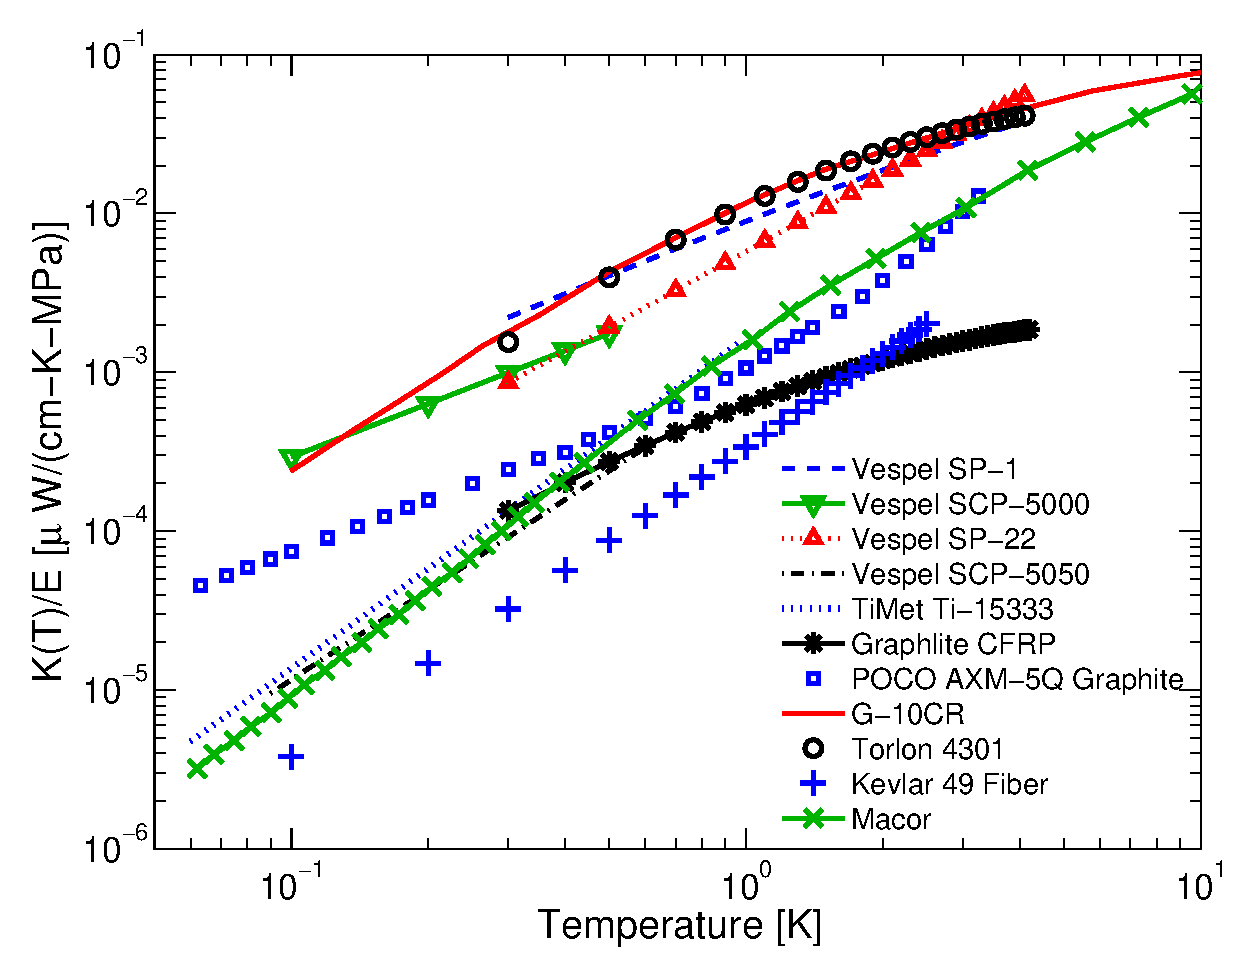
\includegraphics[%
  width=0.65\linewidth,
  keepaspectratio]{Mats}
\end{center}
\caption{A selections of materials with their Youngs modulus normalized by their thermal conductivity.  Lower values correspond to more ideal materials for support structures}
\label{Mats}
\end{figure}

(MATERIAL STRENGHT HERE)

\section{Conclusions}
While many different solutions are available when creating cryogenic support structures, following certain design criteria and avoiding potential pitfalls that compromise structural strength allow for tube and truss structures to remain string while providing low heat loads between stages.  It is important to design with a large factor of safety beyond the theoretical failure point of a structure due to the imperfection dominated failure modes that exist in actual structures of this variety.  When considering truss members, tubes offer high stiffness but little to no elastic region before fracture.  Rods offer more elasticity which makes them susceptible to buckling.

\begin{acknowledgements}
We would like to thank S. Govindjee for technical assistance and use of his strength testing equipment. We acknowledge support and funding from the Department of Energy and the National Science Foundation.
\end{acknowledgements}

\begin{thebibliography}{99}

\bibitem{Gov}
Govindjee note (how do I cite this?)

\bibitem{Hastings}
Peter R. Hastings and D.M. Montgomery. Support of cooled components in astronomical instruments. Cryogenics, 33(11):1032–1036, 1993.

\bibitem{Bazant}
Z. Ba$\check{z}$ant and L. Cedoli. Stability of structures: elastic, inelastic, fracture, and damage theories. Oxford University Press, New York, 1991.

\bibitem{Ely}
R.E. Ely. Strength of graphite tube specimens under combined stresses. Journal of the American Society, 48:505– 508, 1965.

\end{thebibliography}

\end{document}
